% ED2 first journal-program article: authorship and version are NOT finalized.
% Primary published predecessor: QS-Cube/ED (QS^3, CPC 277 (2022) 108369).
% Never assign a CPC accession, software DOI, or credit unconfirmed authors.
\documentclass[preprint,12pt,nopreprintline]{elsarticle}
\usepackage{amsmath,amssymb,bm,booktabs,hyperref}
\usepackage{pgfplots}
\usetikzlibrary{positioning}
\pgfplotsset{compat=1.17}
\hypersetup{colorlinks=true,linkcolor=black,citecolor=blue,urlcolor=blue}
\emergencystretch=2em
\journal{Computer Physics Communications}
\newcommand{\EDtwo}{ED2}
\newcommand{\QSthree}{QS$^{3}$}
\newcommand{\updn}{N_{\downarrow}}
\begin{document}
\begin{frontmatter}
\title{ED2: Generalized exact diagonalization of mixed-spin quantum Hamiltonians with anisotropic and nonconserving interactions}
\author[aff]{Author list pending project approval}
\address[aff]{Affiliations to be confirmed before submission}
\begin{abstract}
We present the first journal-program description of ED2, a Fortran
exact-diagonalization code extending the previously published QS$^3$
spin solver from fixed-magnetization, spin-$1/2$ XXZ models to
generalized Hamiltonians with site-dependent spin magnitudes, anisotropic
exchange, Dzyaloshinskii--Moriya interactions, symmetric off-diagonal
exchange, and vector magnetic fields. Its representation uses
bounded-occupation combinatorics, optional compatible lattice symmetries,
dense and iterative eigensolvers, and Cartesian spin observables.
Physical continuity with the original QS$^3$ executable is verified
through 32 fixed-magnetization eigenvalues, 15 momentum-resolved levels,
and independently referenced conventional-Lanczos calculations for
12--24 sites. In a genuinely non-$U(1)$ alternating spin-$1/2$/spin-$1$
chain, independent Hamiltonian constructions validate calculations
through 12 sites (full Hilbert dimension 46,656).
The staggered vector-chirality response to an oriented DM interaction
agrees with the Hellmann--Feynman energy derivative and independently
computed finite-size susceptibilities. Additional numerical tests probe
near-degenerate states and quantify model-dependent operator-cache
storage. ED2 thus extends the accessible model and observable scope of
the earlier program without claiming a new eigensolver or a previously
unknown magnetic phase.
\end{abstract}
\begin{keyword}
exact diagonalization \sep quantum spin systems \sep mixed spins \sep
Dzyaloshinskii--Moriya interaction \sep Lanczos method \sep reproducible software
\end{keyword}
\end{frontmatter}

\section*{Program summary (provisional; not release metadata)}
\begin{description}\sloppy
\item[Program title:] ED2 (QS$^3$--ED2).
\item[Program version:] To be assigned after integration and release review.
\item[Program repository:] \url{https://github.com/QS-Cube/ED2};
development verification: \url{https://github.com/ueda1984/ED2}.
\item[Previous CPC program:] QS$^3$,
\url{https://github.com/QS-Cube/ED}, Ref.~\cite{ueda2022}.
\item[Program Library accession/DOI:] Not yet assigned.
\item[License:] MIT; copyright and contributor attribution to be verified
against the final distributed release.
\item[Language and dependencies:] Fortran, BLAS/LAPACK, GNU Autotools;
OpenMP is used for shared-memory parallelism.
\item[Unusual features:] Site-dependent mixed spins, oriented
DM and symmetric off-diagonal exchange, complete Cartesian
static correlators, optional Hamiltonian-transition caching
and reproducible numerical-acceptance diagnostics.
\item[Nature of problem:] Finite-size spectra and static spin observables
of spin models with unequal local spins and general bilinear couplings.
\item[Solution method:] Bounded-occupation basis construction,
optional compatible symmetry representations, dense Hermitian
diagonalization or iterative Lanczos-type eigensolvers.
\item[Restrictions:] Exponential Hilbert-space growth. Occupation
windows of nonconserving Hamiltonians generally represent projected
operators rather than exact invariant sectors. The released interface
is an executable, not an installed reusable library ABI.
\end{description}

\section{Introduction}
Exact diagonalization (ED) is a reference method for finite quantum
many-body systems, but the dimension of the full spin Hilbert space
grows as $\mathcal D=\prod_i(2S_i+1)$.
Conservation laws and spatial symmetries can significantly reduce this
dimension. The published \QSthree{} program
of Ueda, Yunoki and Shimokawa~\cite{ueda2022}
targets spin-$1/2$ XXZ-type models near saturation, using fixed
down-spin number, translation/momentum sectors, Lanczos eigensolvers,
static spin observables and a dynamical spin-structure-factor pathway.
Its published source is \url{https://github.com/QS-Cube/ED}.

The present work is the \emph{first journal-program paper for ED2}.
ED2 source has already been available in the distinct
\url{https://github.com/QS-Cube/ED2} repository; that prior public
availability must not be confused with an earlier journal publication.
Relative to the published \QSthree{} code, ED2 extends the represented
local spin spaces and bilinear operators to mixed spins, XYZ anisotropy,
directed Dzyaloshinskii--Moriya (DM) exchange, symmetric off-diagonal
exchange and site-dependent magnetic fields. Total $S^z$ need not be
conserved. ED2 also provides Cartesian one- and two-spin observables.
The original program's numerical solvers and OpenMP methodology
are not claimed as new algorithms, nor is ED2 presented as a strict
feature superset of the original dynamical-response code.

The broader computational ecosystem includes ALPS~\cite{bauer2011},
QuSpin~\cite{weinberg2017} and the H$\Phi$ quantum-lattice solver,
including its later updates~\cite{kawamura2017,ido2024}.
These tools have different numerical designs and supported workflows;
we make no assertion that mixed spins or DM couplings are exclusive
to ED2. The contribution here is instead the documented
\emph{program-specific} extension of the CPC-published QS$^3$
software, its compact Fortran model input and its independently
verified numerical and physical observable contracts.


Table~\ref{tab:program-scope} summarizes scientific scope relative
to the \emph{published} \QSthree{} program, not to the already-public
ED2 repository. The original code retains a dynamical structure-factor
path that has not been verified as a native ED2 capability.
No binary or file-format backward compatibility is asserted.

\begin{table}[t]
\centering
\caption{Main program differences relative to the CPC-published
QS$^3$/ED executable. Neither the underlying eigensolvers nor
the generalized spin-model category are claimed to be exclusive.}
\label{tab:program-scope}
\small
\begin{tabular}{p{0.23\linewidth}p{0.30\linewidth}p{0.34\linewidth}}
\toprule
Capability & QS$^3$/ED (2022) & ED2 \\
\midrule
Local spins & Uniform $S=1/2$ & Site-dependent $S_i$; mixed spins \\
Bond couplings & XXZ-type & XYZ, directed DM, symmetric $\Gamma$ \\
Site fields & Restricted input & Site-dependent Cartesian fields \\
Basis & Fixed $N_\downarrow$ and momentum & Bounded occupations, full space, compatible symmetries \\
Static output & Selected spin channels & Nine Cartesian pair components \\
Dynamic spectra & Dedicated dynamic path & Equivalent native path unverified \\
Solvers & Dense, Lanczos, restarted & Inherited families; revised diagnostics \\
\bottomrule
\end{tabular}
\end{table}

\section{Hamiltonians and Hilbert-space representation}
\subsection{General local operators}
For oriented input bonds $(i,j)$, ED2 represents
\begin{align}
H={}&\sum_{(i,j)}\left[
\sum_{\alpha=x,y,z}J^\alpha_{ij}S_i^\alpha S_j^\alpha
+\bm D_{ij}\cdot(\bm S_i\times\bm S_j)\right.\nonumber\\
&\left.\hspace{13mm}+
\sum_{\alpha=x,y,z}\Gamma^\alpha_{ij}
(S_i^{\beta_\alpha}S_j^{\gamma_\alpha}
 +S_i^{\gamma_\alpha}S_j^{\beta_\alpha})\right]
+\sum_i\bm h_i\cdot\bm S_i ,
\label{eq:general}
\end{align}
where $(\beta_x,\gamma_x)=(y,z)$,
$(\beta_y,\gamma_y)=(z,x)$ and
$(\beta_z,\gamma_z)=(x,y)$.
The input field convention is $+\bm h\cdot\bm S$.
A physical Zeeman field $-\bm B\cdot\bm S$ is therefore
encoded by $\bm h=-\bm B$.
The DM term changes sign under reversal of the oriented bond.
Nine real couplings per bond specify the three diagonal exchanges,
three DM components and three symmetric off-diagonal exchanges.

\subsection{Generalizing the original binomial basis}
In the published spin-$1/2$ XXZ solver, a fixed
$\updn=n$ subspace has dimension $\binom{L}{n}$.
ED2 allows local occupations $n_i=0,\dots,m_i$
with $0\leq m_i\leq 2S_i$. Define
\begin{align}
P_L(x)&=\prod_{i=1}^{L}\left(\sum_{q=0}^{m_i}x^q\right),
&
a_L(n)&=[x^n]P_L(x),\nonumber\\
\mathcal D_{\mathrm{window}}
&=\sum_{n=N_{\min}}^{N_{\max}}a_L(n),
&
a_i(n)&=\sum_{q=0}^{m_i}a_{i-1}(n-q).
\label{eq:occupation}
\end{align}
These are dimensions before spatial-symmetry reduction.
For $m_i=1$, $P_L=(1+x)^L$, recovering the original
binomial representation exactly. The complete local product
space has dimension $P_L(1)=\prod_i(2S_i+1)$.

The allowed occupation window is not automatically a conserved
sector. If $[H,\sum_i S_i^z]\neq0$, restricting occupations
generally defines a projected Hamiltonian $PHP$, not an
exact representation of the original ground-state problem.
Similarly, user-provided site permutations represent physical
symmetry sectors only when they commute with the full Hamiltonian.


\subsection{Program organization}
Figure~\ref{fig:workflow} summarizes the main operations.
Spin and bond input records define the local operator basis
and optionally a symmetry-compatible representation.
The Hamiltonian action is supplied either on demand or
through a configurable transition cache, and the selected
eigensolver passes its states to the observable and numerical
diagnostic stages. The modular depiction describes data flow,
not a distinct newly proposed diagonalization algorithm.

\begin{figure}[t]
\centering
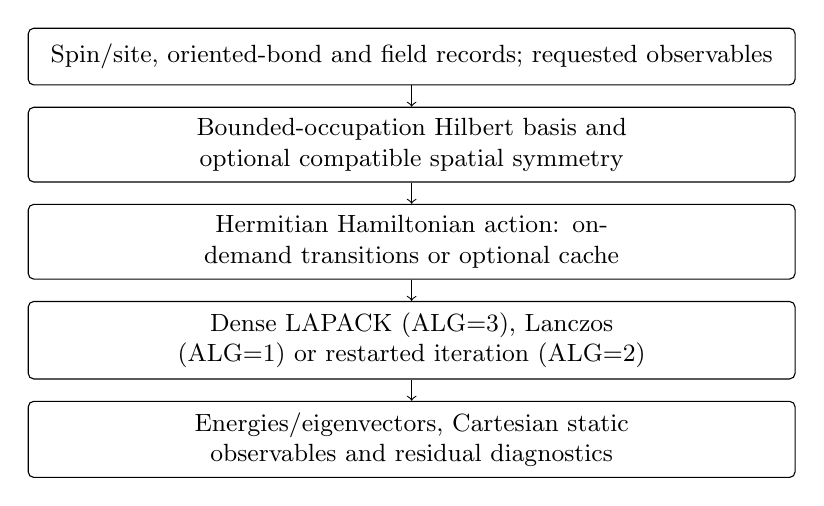
\begin{tikzpicture}[
box/.style={draw,rounded corners=2pt,align=center,
            text width=0.78\linewidth,minimum height=0.72cm,
            inner sep=4pt,font=\small},
node distance=0.27cm
]
\node[box] (inputs) {Spin/site, oriented-bond and field records;
requested observables};
\node[box,below=of inputs] (basis) {Bounded-occupation Hilbert basis
and optional compatible spatial symmetry};
\node[box,below=of basis] (action) {Hermitian Hamiltonian action:
on-demand transitions or optional cache};
\node[box,below=of action] (solver) {Dense LAPACK (ALG=3),
Lanczos (ALG=1) or restarted iteration (ALG=2)};
\node[box,below=of solver] (outputs) {Energies/eigenvectors,
Cartesian static observables and residual diagnostics};
\draw[->] (inputs)--(basis);
\draw[->] (basis)--(action);
\draw[->] (action)--(solver);
\draw[->] (solver)--(outputs);
\end{tikzpicture}
\caption{Program-level data flow. Neither the eigensolver
families nor OpenMP execution are introduced as new algorithms.}
\label{fig:workflow}
\end{figure}

\section{Numerical implementation and validation}
ED2 supports dense Hermitian LAPACK diagonalization (ALG=3),
conventional Lanczos (ALG=1), and restarted Hermitian iteration
(ALG=2). The numerical-development line adds explicit
BLAS/LAPACK interfaces, magnetic-field indexing repairs,
Krylov diagnostics, residual acceptance controls and reproducible
input/source distributions. It does not introduce a new
Lanczos method.

For a normalized Ritz pair $(E,\psi)$, the direct residual
$r=\|H\psi-E\psi\|_2$ is an important numerical diagnostic.
However, a small residual alone does not certify that $E$
is the globally lowest eigenvalue; near degeneracy it cannot
certify an individual state-specific expectation value either.
We therefore compare energy levels, residuals and physical
observables against independently assembled Hamiltonians.

\subsection{Continuity with the published QS$^3$ executable}
The original \QSthree{} source was checked out at
commit \texttt{a3b09934bba5} (full SHA preserved in
the archived verification inputs) and compiled
without modifying its production Fortran. In shared spin-$1/2$,
open-boundary XXZ limits ($J_{xy}=0.8$, $J_z=1.1$),
all 32 eigenvalues across the three invariant sectors
$(L,\updn)=(4,2),(6,1),(6,3)$ agree with ED2 and a separately
constructed sector Hamiltonian. The largest old-to-new
difference is $2.89\times10^{-15}$.

Table~\ref{tab:continuity} gives an additional direct comparison
of the original and ED2 \emph{conventional Lanczos} executables.
Both target the same fixed-$\updn=2$ ground energy at 12--24 sites.
The original implementation uses a random initial vector:
iteration counts and wall times cannot be interpreted as
matched-start performance ratios. Two source-pinned CI repetitions
independently passed against the exact reference, with observed
old-to-new energy differences below $2\times10^{-13}$.

\begin{table}[t]
\centering
\caption{Direct ALG=1 continuity in a common open XXZ sector.
The displayed energies are from the independently referenced
first source-archived execution. Iterations are not matched-start
performance observations.}
\label{tab:continuity}
{\small
\begin{tabular}{rrrrr}
\toprule
$L$ & $\binom{L}{2}$ & $E_0$ (reference)
& $|\delta E_{\mathrm{QS^3}}|$ & $|\delta E_{\mathrm{ED2}}|$\\
\midrule
12 & 66 & -0.62256313375 & $1.11\times10^{-16}$ & 0\\
18 & 153 & 0.94064437307 & $1.99\times10^{-14}$ & $2.11\times10^{-15}$\\
24 & 276 & 2.56129305705 & $1.11\times10^{-14}$ & $8.88\times10^{-16}$\\
\bottomrule
\end{tabular}
}
\end{table}

On a periodic six-site XXZ ring, we independently construct
the translation projector
\begin{equation}
P_m=\frac{1}{L}\sum_{r=0}^{L-1}e^{-2\pi i m r/L}\,T^r.
\end{equation}
It resolves the fixed-$\updn=2$ space into six translation
sectors. Their dimensions are $3,2,3,2,3,2$.
The original \QSthree{} and ED2 executables reproduce
all 15 sector-resolved eigenvalues, with maximum
cross-code difference $3.11\times10^{-15}$.
This validates inherited \emph{static momentum-sector
spectra}; the earlier dynamical-response pathway is not
asserted to have been ported.

\subsection{Independent mixed-spin basis checks}
For $S_i=(1/2,1,1/2,1)$, the polynomial in
Eq.~\eqref{eq:occupation} is
$(1+x)^2(1+x+x^2)^2$.
The full occupation window $[0,6]$ has 36 states;
$[3,3]$ has 10 and $[2,4]$ has 26.
The actual ED2 dense solver reproduces all
72 independently enumerated levels across these three
representations, with maximum absolute difference
$1.11\times10^{-16}$.


\subsection{Independent verification coverage}
The source-pinned tests cover both exact spectra and
computed observables (Table~\ref{tab:validation}).
These numbers establish correctness for the displayed
Hamiltonians and environments, not an exhaustive
verification over arbitrary coupling and boundary inputs.
A small direct residual is necessary for eigenpair
acceptance but cannot by itself identify the global
ground state in a near-degenerate problem.

\begin{table}[t]
\centering
\caption{Verified comparisons to the published executable
or to independently assembled reference Hamiltonians.
Reported maxima refer to different numerical observables.}
\label{tab:validation}
\small
\begin{tabular}{p{0.37\linewidth}r p{0.35\linewidth}}
\toprule
Validation family & Cases & Maximum reported discrepancy \\
\midrule
Original QS$^3$ XXZ spectrum & 32 levels & $2.89\times10^{-15}$ old/new \\
QS$^3$ momentum sectors & 15 levels & $3.11\times10^{-15}$ old/new \\
Mixed-spin bounded basis & 72 levels & $1.11\times10^{-16}$ to reference \\
Staggered-DM response & 60 runs & $<1.4\times10^{-13}$ in $E_0$;
$<1.5\times10^{-9}$ in $K$ \\
Published XYZ--DM conventions & 12 runs & $<3\times10^{-14}$ in spectrum \\
\bottomrule
\end{tabular}
\end{table}


\subsection{Low-energy subspace observables near degeneracy}
When low eigenvalues approach one another, a small
individual Ritz residual is not enough to establish
stable state-specific magnetizations. For a separated
two-state low-energy manifold, we additionally compare
the subspace-averaged observable
\begin{equation}
\overline A_{\rm low}=\frac12\operatorname{Tr}(P_{\rm low}A),
\qquad
P_{\rm low}=\sum_{n=0}^1 |\psi_n\rangle\langle\psi_n|.
\label{eq:projector}
\end{equation}
This is invariant under a unitary rotation of the
two basis vectors spanning the same projector.
An interacting eight-site sparse doublet test
compared native ED2 wavefunctions with an independently
constructed reference projector: 20/20 runs passed,
with the largest reported trace-observable difference
below $3.75\times10^{-10}$.
A separate numerical stress test with first gaps
of order $10^{-7}$ accepted 24/24 runs; the low-doublet
correlation traces differed by at most about
$2.26\times10^{-9}$ from the sparse reference.
Dense-LAPACK and perturbative-reference crosschecks
also show why a near-degenerate reference eigenvector
cannot automatically be regarded as exact.
These are numerical robustness tests, not claims
of arbitrary-precision state certification.

\section{Scientific example: staggered vector chirality}
Consider an open, alternating spin-$1/2$/spin-$1$ chain
with $S_{2i-1}=1/2$ and $S_{2i}=1$.
For zero-based site/bond index $j$ let
$\eta_j=(-1)^j$, and define
\begin{align}
H(D)&=H_0+D\hat K,\label{eq:hdm}\\
\hat K&=\sum_{j=0}^{L-2}
\eta_j(S_j^xS_{j+1}^y-S_j^yS_{j+1}^x).
\label{eq:chirality}
\end{align}
The baseline $H_0$ retains the non-$U(1)$ terms
$J_j^\alpha S_j^\alpha S_{j+1}^\alpha$,
$\Gamma^z_j(S_j^xS_{j+1}^y+S_j^yS_{j+1}^x)$,
and $h_j^x S_j^x+h_j^z S_j^z$, with a fixed
two-site periodic coefficient rule:
\begin{align}
J_j^x&=0.77+0.05\eta_j,& J_j^y&=0.63+0.03\eta_j,\nonumber\\
J_j^z&=1.09-0.04\eta_j,& \Gamma_j^z&=0.065+0.015\eta_j,\nonumber\\
h_j^x&=0.15(0.4\eta_j+0.1),&
h_j^z&=0.17+0.035\eta_j.
\label{eq:coefficients}
\end{align}
For fields $\eta_j$ is the site parity; for bonds
it is the parity of the bond's first site.
The complete $L=12$ Hilbert space contains
$6^{L/2}=46{,}656$ states and is treated without
a fixed-magnetization projection.

For a nondegenerate ground state,
\begin{equation}
\frac{\partial E_0}{\partial D}=\langle\hat K\rangle,
\qquad
\bar\kappa_{\mathrm{stag}}=\frac{\langle\hat K\rangle}{L-1}.
\label{eq:hf}
\end{equation}
Independently evaluated energy differences, direct
chirality operators and ED2's $xy-yx$ Cartesian
two-spin correlation outputs agree. The ordering
of those output components is explicitly audited
to detect $xy/yx$ sign swaps.
The finite-size susceptibility is
\begin{equation}
\chi_\kappa(L)=-\frac{1}{L-1}
\left.\frac{\partial^2E_0}{\partial D^2}\right|_{D=0},
\label{eq:susc}
\end{equation}
also checked by finite differencing $\langle\hat K\rangle$.
For $L=4,6$, full spectral sums provide an additional
independent reference. Table~\ref{tab:susc} reports the results.

\begin{table}[t]
\centering
\caption{Finite-size, bond-normalized staggered chirality susceptibility
of the explicitly specified alternating-spin model. These values
are not thermodynamic-limit extrapolations.}
\label{tab:susc}
\begin{tabular}{rr}
\toprule
$L$ & $\chi_\kappa(L)$\\
\midrule
4 & 0.634311\\
6 & 0.568733\\
8 & 0.537355\\
10 & 0.519701\\
12 & 0.508501\\
\bottomrule
\end{tabular}
\end{table}


% DATA PROVENANCE: docs/development/cpc-stationary-dm-reference.csv
% Five D points for each L; re-verify against source CSV after any edit.
\begin{figure}[t]
\centering
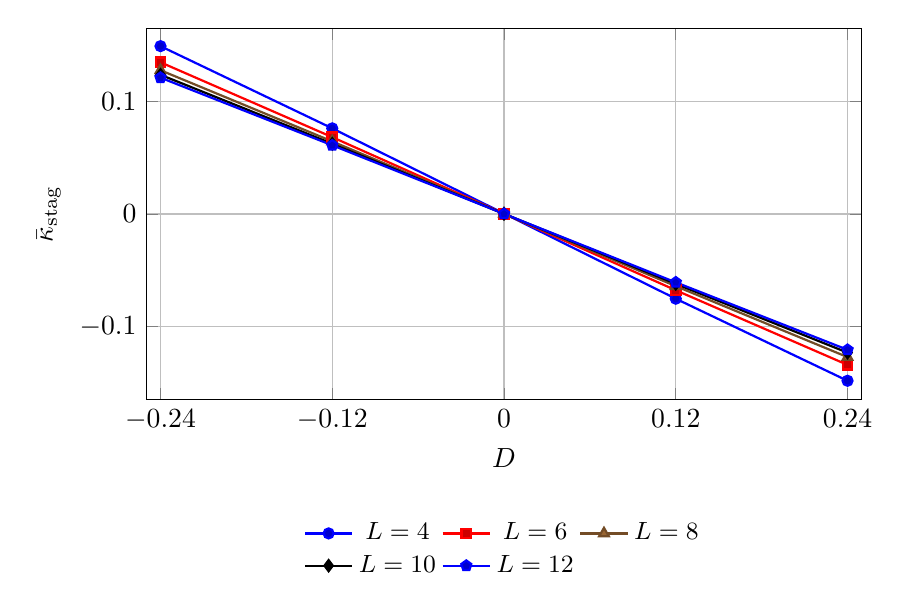
\begin{tikzpicture}
\begin{axis}[
 width=0.88\linewidth, height=6.3cm,
 xmin=-0.25, xmax=0.25, ymin=-0.165, ymax=0.165,
 xlabel={$D$},
 ylabel={$\bar\kappa_{\mathrm{stag}}$},
 xtick={-0.24,-0.12,0,0.12,0.24},
 grid=major,
 legend columns=3,
 legend style={at={(0.5,-0.30)},anchor=north,draw=none,font=\small}
]
\addplot+[mark=*,mark size=1.8pt,thick] coordinates {(-0.24,0.1490669111) (-0.12,0.07606183469) (0,0.0003834158887) (0.12,-0.0752541082) (0.24,-0.1481511796)};
\addlegendentry{$L=4$}
\addplot+[mark=square*,mark size=1.7pt,thick] coordinates {(-0.24,0.1347374411) (-0.12,0.06823183021) (0,0.0002180106964) (0.12,-0.06773345395) (0.24,-0.1340445297)};
\addlegendentry{$L=6$}
\addplot+[mark=triangle*,mark size=2pt,thick] coordinates {(-0.24,0.127667629) (-0.12,0.06446533643) (0,0.0001562908303) (0.12,-0.06409869328) (0.24,-0.1271197533)};
\addlegendentry{$L=8$}
\addplot+[mark=diamond*,mark size=2pt,thick] coordinates {(-0.24,0.1236346982) (-0.12,0.0623495264) (0,0.0001334762108) (0.12,-0.06203513532) (0.24,-0.1231565869)};
\addlegendentry{$L=10$}
\addplot+[mark=pentagon*,mark size=1.9pt,thick] coordinates {(-0.24,0.1210662392) (-0.12,0.06100992836) (0,0.0001230441888) (0.12,-0.06072012735) (0.24,-0.1206238829)};
\addlegendentry{$L=12$}
\end{axis}
\end{tikzpicture}
\caption{Finite-size mean staggered vector chirality per bond versus
the oriented DM coupling for the same two-site-periodic alternating-spin
Hamiltonian at all five lengths. The 25 points originate from the
independently validated stationary-DM reference CSV; lines are visual
guides, not bulk-limit fits.}
\label{fig:dm-response}
\end{figure}


The independent first excitation gaps at the same 25 finite-size
parameter points are displayed in Fig.~\ref{fig:dm-gap}.
All reported gaps are strictly positive on the sampled finite
chains, but these data neither establish a bulk spin gap
nor identify a phase boundary.
Figure~\ref{fig:dm-susceptibility} shows the five $D=0$
susceptibilities from Table~\ref{tab:susc}.
We do not extrapolate them to a thermodynamic limit.

% DATA PROVENANCE: first_gap column, docs/development/cpc-stationary-dm-reference.csv
\begin{figure}[t]
\centering
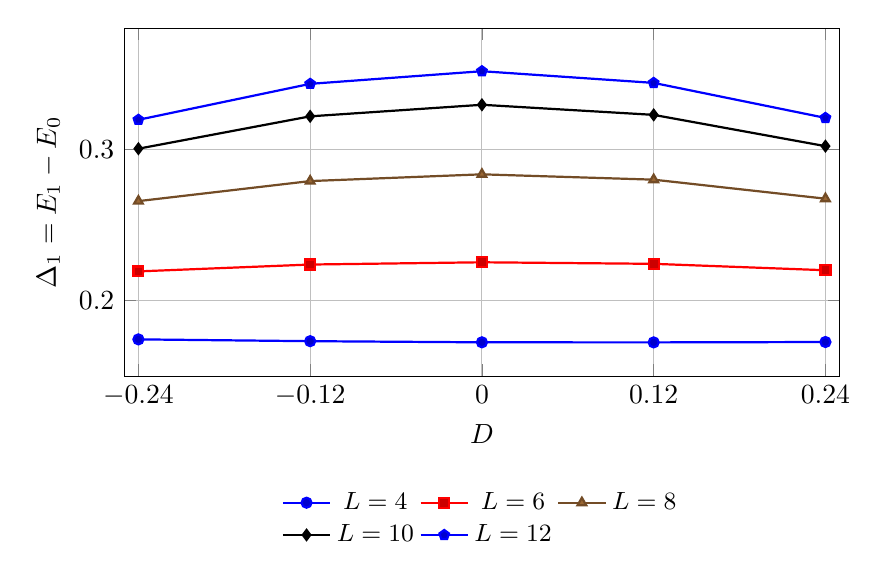
\begin{tikzpicture}
\begin{axis}[
 width=0.88\linewidth, height=6.0cm,
 xmin=-0.25, xmax=0.25, ymin=0.15, ymax=0.38,
 xlabel={$D$}, ylabel={$\Delta_1=E_1-E_0$},
 xtick={-0.24,-0.12,0,0.12,0.24},
 grid=major,
 legend columns=3,
 legend style={at={(0.5,-0.30)},anchor=north,draw=none,font=\small}
]
\addplot+[mark=*,mark size=1.8pt,thick] coordinates {(-0.24,0.17429542) (-0.12,0.17310422) (0,0.17235306) (0.12,0.17230144) (0.24,0.17255018)};
\addlegendentry{$L=4$}
\addplot+[mark=square*,mark size=1.8pt,thick] coordinates {(-0.24,0.2192335) (-0.12,0.22377147) (0,0.22526115) (0.12,0.22424038) (0.24,0.22000646)};
\addlegendentry{$L=6$}
\addplot+[mark=triangle*,mark size=1.8pt,thick] coordinates {(-0.24,0.26569524) (-0.12,0.27894845) (0,0.28340937) (0.12,0.27988068) (0.24,0.26730885)};
\addlegendentry{$L=8$}
\addplot+[mark=diamond*,mark size=1.8pt,thick] coordinates {(-0.24,0.30035433) (-0.12,0.32174582) (0,0.32938732) (0.12,0.32272129) (0.24,0.30203398)};
\addlegendentry{$L=10$}
\addplot+[mark=pentagon*,mark size=1.8pt,thick] coordinates {(-0.24,0.31946093) (-0.12,0.34321831) (0,0.35158094) (0.12,0.34385254) (0.24,0.32070682)};
\addlegendentry{$L=12$}
\end{axis}
\end{tikzpicture}
\caption{First excitation gaps of the same alternating-spin
Hamiltonian at the 25 independently verified finite-size
parameter points. Connecting lines are visual guides;
no thermodynamic extrapolation is made.}
\label{fig:dm-gap}
\end{figure}

% DATA PROVENANCE: chi_kappa_per_bond at D=0 in the same reference CSV
\begin{figure}[t]
\centering
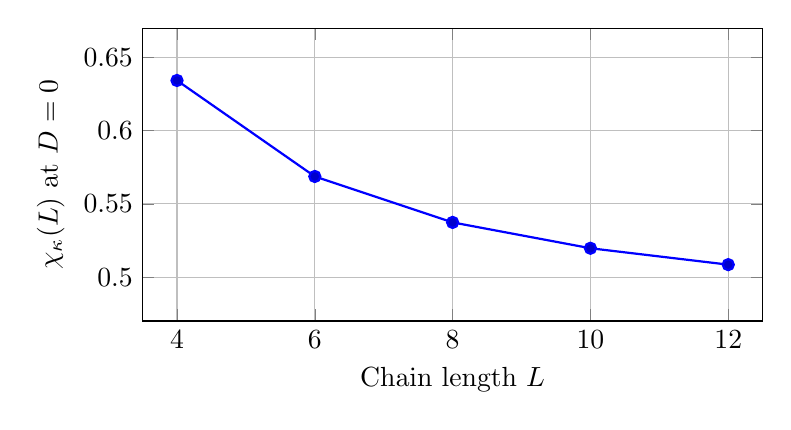
\begin{tikzpicture}
\begin{axis}[
 width=0.78\linewidth, height=5.3cm,
 xmin=3.5, xmax=12.5, ymin=0.47, ymax=0.67,
 xlabel={Chain length $L$},
 ylabel={$\chi_\kappa(L)$ at $D=0$},
 xtick={4,6,8,10,12},
 grid=major
]
\addplot+[mark=*,mark size=2pt,thick] coordinates {(4,0.6343112017685585) (6,0.5687329253277751) (8,0.5373552578573756) (10,0.5197013169818259) (12,0.5085009862217026)};
\end{axis}
\end{tikzpicture}
\caption{Bond-normalized finite-size staggered-chirality
susceptibility at $D=0$, Eq.~\eqref{eq:susc}.
Its length dependence does not establish a bulk value
or critical exponent.}
\label{fig:dm-susceptibility}
\end{figure}

The 60 source-archived, independent OMP=1/2 checks through
12 sites reproduce ground energies and full nearest-neighbor
Cartesian correlators. The calculated smooth finite-size response
does not establish a chiral phase transition or a reliable
thermodynamic extrapolation. A separate validation checks a
properly converted finite-size Hamiltonian from the XYZ/DM
literature~\cite{yi2019}; it is not a reproduction
of a published phase diagram. Alternating-spin DM
models have also been studied elsewhere~\cite{lahiri2022},
but the coefficients in Eq.~\eqref{eq:coefficients}
were chosen as a software-validation example
rather than copied from that literature.


\subsection{Hamiltonian-level reproduction of a published XYZ--DM model}
A second, spin-$1/2$ validation reconstructs the periodic
XYZ--DM Hamiltonian of Yi \emph{et al.}~\cite{yi2019},
written there in terms of Pauli matrices
$\sigma^\alpha=2S^\alpha$. The exact coefficient
conversion to ED2 is
\begin{equation}
\begin{split}
J_x&=2J(1+\gamma),\quad J_y=2J(1-\gamma),
\quad J_z=4J\Delta,\\
D_z&=4D_{\rm Y},\qquad h_z=-2h.
\end{split}
\label{eq:pauli-conversion}
\end{equation}
The periodic closing bond must also retain its directed
DM orientation. For $J=1$, $\gamma=0.37$,
$\Delta=0.41$, and $h=0.58$, the six independent
reference values in Table~\ref{tab:literature}
are reproduced by ED2 with one and two OpenMP threads.
The complete spectrum matches independent Pauli
construction within $3\times10^{-14}$.
Cartesian correlators and the DM-conjugate expectation
also agree within $10^{-14}$. These are
\emph{finite-size Hamiltonian-level} consistency
checks at chosen test parameters, not a reproduction
of numerical points or phase boundaries in Ref.~\cite{yi2019}.

\begin{table}[t]
\centering
\caption{Independent ground energies and first excitation gaps
for the published periodic spin-$1/2$ XYZ--DM Hamiltonian.
Here $D_{\rm Y}$ denotes the Pauli-matrix DM coefficient.}
\label{tab:literature}
\small
\begin{tabular}{rrrr}
\toprule
$L$ & $D_{\rm Y}$ & $E_0$ & $E_1-E_0$\\
\midrule
4 & 0.00 & -3.854733105562 & 0.478797061\\
4 & 0.19 & -3.854733105562 & 0.478797061\\
6 & 0.00 & -5.466704725748 & 0.006836479\\
6 & 0.19 & -5.468567485505 & 0.008699239\\
8 & 0.00 & -7.368761434736 & 0.172597665\\
8 & 0.19 & -7.369394757989 & 0.170241793\\
\bottomrule
\end{tabular}
\end{table}

\section{Cache storage and performance limitations}
The existing ED2 cache controls \texttt{wk\_dim} and \texttt{MNTE}
trade stored Hamiltonian transitions against on-demand work.
For the stationary alternating chain in Sec.~5,
the independently checked exact maximum number of nontrivial
entries per row is $\mathrm{MNTE}=7L/2-1$.
The default broad capacity is $10L-7$ \emph{allocated}
entries per row including the diagonal/spare slot convention.
On the tested LP64 representation, each cached
entry uses one 4-byte index and one 16-byte complex
amplitude, giving the corresponding nominal cache
allocation formulas
\begin{align}
B_{\mathrm{half,generic}}&=
20(10L-7)\left\lfloor\mathcal D/2\right\rfloor,\nonumber\\
B_{\mathrm{full,tight}}&=
20(7L/2)\mathcal D,\nonumber\\
B_{\mathrm{full,generic}}&=
20(10L-7)\mathcal D.
\label{eq:cache}
\end{align}
At $L=12$ these are respectively 50.279,
37.375 and 100.558 MiB \emph{of cache arrays},
not total process resident memory.
The full/tight cache can therefore store all rows while
using less cache-array memory than half/generic for this model.
This row bound is not asserted for arbitrary Hamiltonians.


Table~\ref{tab:cache-resource} compares the analytic
cache-array allocation with measured peak resident memory
for the same $L=12$, ALG=1, one-thread workload at
$D=0.12$. Every configuration uses 140 Hamiltonian
applications and passes the independent energy,
correlator and residual checks. The RSS numbers are
observations from a shared GitHub Actions runner;
they are \emph{not} claimed as portable performance bounds.

\begin{table}[t]
\centering
\caption{Model-specific $L=12$ cache-array allocation
and exploratory peak RSS. The analytic allocation
excludes vectors, runtime and allocator overhead.
Measured RSS is not a dedicated-node benchmark.}
\label{tab:cache-resource}
\small
\begin{tabular}{lrr}
\toprule
Cache policy & Cache arrays (MiB) & Peak RSS (KiB) \\
\midrule
Half / generic & 50.279 & 67,970\\
Full / tight & 37.375 & 54,886\\
Full / generic & 100.558 & 119,516\\
\bottomrule
\end{tabular}
\end{table}

The accompanying CI-based resource tests independently check
energies, observables and direct residuals across cache policies,
including observed peak RSS and Hamiltonian applications.
Those shared-runner wall times are exploratory; the program's
publication benchmark requires exclusive-node,
CPU-pinned, repeated measurements and operator
verification of hardware exclusivity. No general speedup
or parallel efficiency is claimed here.


\section{User workflow and reproducibility}
ED2 is currently distributed as a Fortran executable
\texttt{source/QS3ED2}, not as a stable installed library.
For the examples in this article the input records specify
on-site spins, oriented bonds with their couplings, fields
and requested Cartesian correlations. The output includes
low energies, magnetizations and nine component-resolved
two-site correlators. The ordering in
\texttt{two\_body\_cf\_xyz.dat} is
$(xx,yx,zx,xy,yy,zy,xz,yz,zz)$ rather than
the usual row-major ordering; the operator-conjugate
$xy-yx$ check is designed to catch an inadvertent swap.

For a Linux environment with GNU Fortran, GNU Autotools
and BLAS/LAPACK, the $L=4$ physical example can be
regenerated from a reviewed checkout with the following
commands (all output paths must be fresh):
\begin{verbatim}
autoreconf -vfi
./configure FC=gfortran FCFLAGS="-O2 -fopenmp"
make -j2
export OPENBLAS_NUM_THREADS=1
python3 -S tests/cpc_portable_dm_quickstart.py \
  --exe "$(pwd)/source/QS3ED2" \
  --size 4 --omp 1 \
  --output "$(pwd)/ed2-reproduction-l4"
\end{verbatim}
This driver constructs the input decks, runs ED2
at three nearby DM strengths and checks the native
correlation-derived chirality and finite-difference
susceptibility against frozen independent references.
It uses only the Python standard library \emph{after}
building the Fortran executable. The full independent
physics tests instead require NumPy/SciPy to construct
separate dense/sparse spin Hamiltonians.
The source archive and development repository retain
the input recipes, reference CSV and workflow definitions.

The final CPC program package must replace the moving
branch with a full immutable source SHA or release tag,
author-approved version and source archive, compiler
and numerical-library provenance, and representative
input/output files. The software DOI and Program Library
accession are not assigned in this draft.

\section{Availability and limitations}
The public source lineage is
\url{https://github.com/QS-Cube/ED2};
development verification is archived under
\url{https://github.com/ueda1984/ED2}.
Build and test scripts reproduce the original
source-pinned QS$^3$ overlap, stationary mixed-spin
DM response, independent low-energy references
and model-specific memory accounting.
The eventual official merged release, archive version,
CPC Program Library accession, software DOI and complete
authorship/credit require project approval and
must be specified before submission.
The old program's dynamical spin-structure-factor pathway
is not verified as a native ED2 capability.

\section{Conclusions}
ED2 generalizes the published QS$^3$ program's
spin-$1/2$ XXZ computational setting to mixed local
spins and nonconserving anisotropic bilinear operators.
Direct original-code comparisons establish continuity
in both conserved subspaces and translation sectors,
while independent physical-response and numerical
acceptance tests demonstrate the broader executable
model/observable interface. The software remains
subject to finite-size growth and model-dependent
resource costs. The results do not imply a new
eigensolver, a universal performance improvement
or an undiscovered magnetic phase.

\begin{thebibliography}{9}
\bibitem{ueda2022}
H. Ueda, S. Yunoki and T. Shimokawa,
Quantum spin solver near saturation: QS$^3$,
Comput. Phys. Commun. \textbf{277}, 108369 (2022).
\href{https://doi.org/10.1016/j.cpc.2022.108369}{doi:10.1016/j.cpc.2022.108369}.
\bibitem{yi2019}
T.-C. Yi, W.-L. You, N. Wu and A. M. Ole\'s,
Criticality and factorization in the Heisenberg chain with
Dzyaloshinskii--Moriya interaction,
Phys. Rev. B \textbf{100}, 024423 (2019).
\href{https://doi.org/10.1103/PhysRevB.100.024423}{doi:10.1103/PhysRevB.100.024423}.
\bibitem{lahiri2022}
A. Lahiri and S. K. Pati,
Loss of classicality in alternating spin-$1/2$/spin-$1$ chain
in the presence of next-neighbor couplings and
Dzyaloshinskii--Moriya interactions,
J. Phys.: Condens. Matter \textbf{34}, 175802 (2022).
\href{https://doi.org/10.1088/1361-648X/ac4aab}{doi:10.1088/1361-648X/ac4aab}.
\bibitem{weinberg2017}
P. Weinberg and M. Bukov,
QuSpin: a Python package for dynamics and exact diagonalisation of quantum many body systems,
SciPost Phys. \textbf{2}, 003 (2017).

\bibitem{bauer2011}
B. Bauer \emph{et al.},
The ALPS project release 2.0: open source software for
strongly correlated systems,
J. Stat. Mech. (2011) P05001.
\href{https://doi.org/10.1088/1742-5468/2011/05/P05001}
{doi:10.1088/1742-5468/2011/05/P05001}.
\bibitem{kawamura2017}
M. Kawamura, K. Yoshimi, T. Misawa, Y. Yamaji,
S. Todo and N. Kawashima,
Quantum lattice model solver H$\Phi$,
Comput. Phys. Commun. \textbf{217}, 180--192 (2017).
\href{https://doi.org/10.1016/j.cpc.2017.04.006}
{doi:10.1016/j.cpc.2017.04.006}.
\bibitem{ido2024}
K. Ido, M. Kawamura, Y. Motoyama, K. Yoshimi,
Y. Yamaji, S. Todo, N. Kawashima and T. Misawa,
Update of H$\Phi$: Newly added functions and methods
in versions 2 and 3,
Comput. Phys. Commun. \textbf{298}, 109093 (2024).
\href{https://doi.org/10.1016/j.cpc.2024.109093}
{doi:10.1016/j.cpc.2024.109093}.
\end{thebibliography}
\end{document}
